% !TeX root = ../main.tex
% Add the above to each chapter to make compiling the PDF easier in some editors.

\chapter{Distributed Baum-Welch}\label{chapter:hmm-dist}

Learning Hidden Markov Model parameters using the Baum-Welch algorithm can be resource intensive, especially if there is a large amount of training data. One approach to tackling such a problem is to do the computation in a distributed way. That is having multiple computers each work on part of the problem. In addition to the time series generation tool, this paper will also contain a distributed implementation of the Baum-Welch algorithm. 

\section{Apache Spark}

While not impossible, it would be very difficult to create a distributed program like this from scratch. Certainly it would be to much for a paper like this. This is where distributed computing frameworks come in that do a lot of the work for you. 

In this paper the distributed computing framework of choice is Apache Spark. Spark is an open-source distributed general-purpose cluster-computing framework. There are many reasons to chose Spark, one being performance. Spark uses a state-of-the-art DAG scheduler, query optimizer, and physical execution engine. Spark also offers in memory processing to avoid writing to disk. These technologies cause Spark to complete tasks up to 100 times faster that its alternatives for example Hadoop. 

Spark is also has a lot of general applicability. Using various libraries on top of Spark it can be used in various scenarios. For example Spark SQL for queries, MLib for machine learning applications, GraphX for Graph operations, and Spark Streaming for streaming instead of batch operations. 

However the most important reason to chose it for this project is Spark's ease of use. Spark has API in many languages like Java, Scala, Python, R, and SQL. Since we already have a python implementation, the Python API called pyspark is a great choice. In all these languages the API is high-level making it simple to create distributed computation code. (Refernce)

The most important concept in Spark are Resilient Distributed Datasets (RDDs). They are fault tolerant collection of data which is operated on in parallel. There are two types of operations on RDDs: transformations and actions. Transformations create a new dataset from the original. An example of a transformation is "map". "map" applies a function to every member of a dataset. The result of this is a new dataset. An action returns a value after running over the dataset. An example for an action is "reduce". "reduce" aggregates the elements of the dataset using some function and returns the result. (Reference rdd programming guide)

\section{Baum-Welch}
\label{section:distributed-hmm}

\begin{figure}
  \centering
  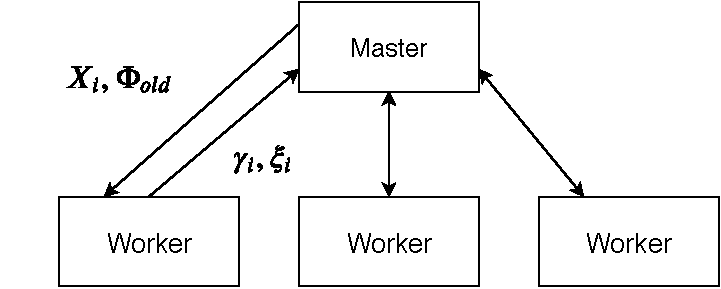
\includegraphics{figures/distributed.pdf}
  \caption{Distributed Baum-Welch}
  \label{fig:distributed}
\end{figure}

Having chosen the appropriate framework for facilitating the distributed computing, now the question is how to split up the work load of the Baum-Welch algorithm so that we actually have work to distribute. 

The opportunity for parallelization comes during the E-step, when dealing with multiple training time-series. For each of them we execute the forward and backward algorithm and compute the intermediate values $\gamma$ and $\xi$. After these are computed for every time-series the intermediate variables get summed up and finally in the M-step they are the basis for new parameters. 

The distributed computation is visualized in Figure \ref{fig:distributed}. During each iteration the master sends a worker a time-series together with the current parameters $\phi$. The workers execute the E-step and returns $\gamma$ and $\xi$ to the master, who once all the results from the workers are in executes the M-step. Note that when programming in pyspark we do not have to worry about masters and workers. The pyspark API abstracts all this away. We just have to think in terms of functional programming. This operation can be achieved using "map" and "reduce". Still Figure \ref{fig:distributed} is helpful in visualizing what is going on. 

\section{Spark Implementation}

As mentioned before the Python Spark API pyspark is very high-level. This means that most of the Baum-Welch implementation from the time-series generation tool can be used as is. The differences come from setting up the Resiliant Distributed Dataset that Spark can then work on. 

\begin{figure}
\begin{singlespace}
\begin{lstlisting}[language=Python]
def fit(X, components, iterations):
    with pyspark.SparkContext("local", "HMM") as sc:
        means, cov, startprop, transmat = init(components, X)
        for i in range(iterations):
            dataobjs = []
            for A in X:
                obj = {}
                obj["data"] = A
                obj["means"] = means
                obj["cov"] = cov
                obj["startprop"] = startprop
                obj["transmat"] = transmat
                obj["components"] = components
                dataobjs += [obj]
            # parallelize into 2 parts
            pardataobjs = sc.parallelize(dataobjs, 2)
            processed = pardataobjs.map(process)
            interm = processed.reduce(sum_intem_values)

            e_start = interm["e_start"]
            e_sumgamma = interm["e_sumgamma"]
            e_xgammasum = interm["e_xgammasum"]
            e_xgammasumsquared = interm["e_xgammasumsquared"]
            e_trans = interm["e_trans"]
            startprop, transmat, means, cov = update_params(e_sumgamma, \
               e_xgammasum, e_xgammasumsquared, e_start, e_trans)
        return startprop, transmat, means, cov
\end{lstlisting}
\end{singlespace}
\caption{Pyspark fit function}    
\label{fig:pyspark-fit-listing}
\end{figure}

Figure \ref{fig:pyspark-fit-listing} shows the implementation of the fit function for the distributed Baum-Welch algorithm. The function signature is the same with the parameters X, components, and iterations. X is the training data, components is the number of hidden states and iterations is the number of iteration of the EM-algorithm. 

First the parameters of the HMM get initialized in the same way as the regular code. Then the main loop follows applying the specified number of iterations. Then comes the E-step which is where the differences start. We set up an array of "dataobjs", one for each time-series in the training data set. The objects each contain a "data" entry which contains the time-series. Additionally they also have entries for all the current parameters of the HMM. 

Now we set up the Resilient Distributed Dataset. An RDD can be created from any collection of data, in this case it is a python array. In line 16 using the Spark Context we call parallelize on the dataobjs array which turns it into an RDD. For the sake of example in this case it is split into two parts. 

Having created the RDD next we want to apply the E-step on each of its entries. This happens through the RDD operation "map". This causes the function "process" to be applied to every RDD entry creating a new RDD "processed" containing the results. 

Next we have to sum up the intermediate values to prepare for the M-step. This is achieved by the RDD operation "reduce". This goes through the "processed" RDD and accumulates the intermediate values according to the function "sum\_interm\_values". "reduce" returns the "interm" obj from which we extract the intermediate values of the E-step. Since we are considering a semi-continuos HMM, there is not just $\gamma$ and $\xi$, but the same 5 intermediate values that we already observed in the E-step in the regular Baum-Welch implementation. 

Finally the M-step is executed through the function "update\_params" just as before. 

\begin{figure}
\begin{singlespace}
\begin{lstlisting}[language=Python]
def sum_intem_values(a, c):
   resultobj = {}
   resultobj["e_start"] = a["e_start"] + c["e_start"]
   resultobj["e_sumgamma"] = a["e_sumgamma"] + c["e_sumgamma"]
   resultobj["e_xgammasum"] = a["e_xgammasum"] + c["e_xgammasum"]
   resultobj["e_xgammasumsquared"] = a["e_xgammasumsquared"] + \
      c["e_xgammasumsquared"]
   resultobj["e_trans"] = a["e_trans"] + c["e_trans"]
   return resultobj
\end{lstlisting}
\end{singlespace}
\caption{Pyspark sum\_interm\_values function}    
\label{fig:pyspark-sum-listing}
\end{figure}

Figure \ref{fig:pyspark-sum-listing} show the code for the "sum\_interm\_values" function. It simply adds together the entries of the two given objects into a result object. 

\begin{figure}
\begin{singlespace}
\begin{lstlisting}[language=Python]
def process(dataobj):
   X = dataobj["data"]
   means = dataobj["means"]
   cov = dataobj["cov"]
   startprop = dataobj["startprop"]
   transmat = dataobj["transmat"]
   k = dataobj["components"]

   n = len(X)
   loglikelihood = log_likelihood(X, k, means, cov)
   logalpha = forward(loglikelihood, startprop, transmat)
   logbeta = backward(loglikelihood, transmat)
   loggamma = logalpha + logbeta
   gamma = lognormalize_gamma(loggamma)

   e_start = gamma[0]
   e_sumgamma = np.einsum("ij->j", gamma)
   e_xgammasum = np.dot(gamma.T, X)
   e_xgammasumsquared = np.dot(gamma.T, X**2)

   e_trans = np.zeros((k, k))
   if n > 1:
      logtrans = compute_trans(
         logalpha, logbeta, loglikelihood, transmat)
      e_trans = np.exp(logtrans)

   resultobj = {}
   resultobj["e_start"] = e_start
   resultobj["e_sumgamma"] = e_sumgamma
   resultobj["e_xgammasum"] = e_xgammasum
   resultobj["e_xgammasumsquared"] = e_xgammasumsquared
   resultobj["e_trans"] = e_trans

   return resultobj
\end{lstlisting}
\end{singlespace}
\caption{Pyspark process function}    
\label{fig:pyspark-process-listing}
\end{figure}

Figure \ref{fig:pyspark-process-listing} show the "process" function. First it extracts its parameters from the single parameter object "dataobj". Then it performs the regular E-step on its given time series by executing the forward and backward algorithm and then computing the necessary intermediate values. Then it assembles them in a resultobj and returns it. These result objects will be the entries of the new processed RDD.